\documentclass[11pt,a4paper]{article}
\usepackage[english]{babel}
\usepackage[utf8]{inputenc}
\usepackage{amsmath, amssymb}
\usepackage{graphicx}
\usepackage{caption}
\usepackage{float}
\usepackage[top=1in, left=1.25in, right=1.25in, bottom=.8in]{geometry}
\usepackage[numbered,framed]{matlab-prettifier}
\usepackage{filecontents}
\usepackage[T1]{fontenc}
\usepackage{bigfoot}
\usepackage{listings}

\numberwithin{equation}{subsection}
\newcommand{\eqname}[1]{\tag*{#1}}

\begin{filecontents*}{h4a.m}
%% Load cropped images
close all; clear all; clc
A=[];
baseDir='CroppedYale/yaleB';
for k= 1:39
    if k<10
        fileDir = strcat(baseDir, '0', num2str(k), '/');
    else
        fileDir = strcat(baseDir, num2str(k), '/');
    end
    fileName = dir(strcat(fileDir, '*.pgm'));
    for kk =1:length(fileName)
        fileRead = imread(strcat(fileDir, fileName(kk).name));
        fileRead = fileRead(:);
        A = [A, fileRead];
    end
end
A=double(A);
% Subtract mean
[m, n]=size(A);
A = A - repmat(mean(A, 1), m, 1);

%% Apply SVD to the matrix of cropped images
[U, S, V] = svd(A, 'econ'); 
% Graphical interpretation of U, S and V

%% plot S
figure(1)
subplot(2,2,1), plot(diag(S), 'ro', 'Linewidth', 1);
xlabel('Modes'); ylabel('Energy Captured')
title('(a) Singular Value Spectrum of Cropped Images')
set(gca, 'Fontsize', 12)
subplot(2,2,2), semilogy(diag(S), 'ro', 'Linewidth', 1);
xlabel('Modes'); ylabel('(log) Energy Captured')
title('(b) Log of Singular Value Spectrum of Cropped Images')
set(gca, 'Fontsize', 12)
subplot(2, 1, 2), plot((diag(S)*100)/sum(diag(S)), 'ro', 'Linewidth', 1);
xlabel('Modes'); ylabel('% of Energy Captured')
title('(c) Singular Value Percentage Spectrum of Cropped Images')
set(gca, 'Fontsize', 12)

%% plot U
figure(2)
for k=1:10
    face=reshape(U(:, k), [192 , 168]);
    subplot(2, 5, k), pcolor(flipud(face)); shading interp;
    title(strcat('Mode ', num2str(k)))
end

%% plot V
figure(3)
for k=1:10
    vect= V(:, k);
    subplot(2, 5, k), plot(vect)
    title(strcat('Mode ', num2str(k)))
end

%% Reconstruct the face image of first mode with specified rank (r) value
r=[1 10 50 100 250 500 1000 1500 2000 2414];
figure(4)
for kk=1:length(r)
    A_res = U(:, 1:r(kk)) * S(1:r(kk), 1:r(kk)) * V(:, 1:r(kk))';
    face_res = reshape(A_res(:, 1), [192 168]);
    subplot(2, 5, kk), pcolor(flipud(face_res)); shading interp;
    title(strcat('Rank ', num2str(r(kk))))
end


%% Load uncropped images
M = [];
baseDir='yalefaces/';
for k= 1:15
    if k<10
        fileDir = strcat(baseDir, 'subject0', num2str(k), '.*');
    else
        fileDir = strcat(baseDir, 'subject', num2str(k), '.*');
    end
    fileName = dir(fileDir);
    for kk =1:length(fileName)
        fileRead = imread(strcat(baseDir, fileName(kk).name));
        fileRead = fileRead(:);
        M = [M, fileRead];
    end
end
M=double(M);
% Subtract mean
[m, n]=size(M);
M = M - repmat(mean(M, 1), m, 1);

%% Apply SVD to the matrix of uncropped images
[u, s, v] = svd(M, 'econ'); 
% Graphical interpretation of u, s and v

%% plot s
figure(6)
subplot(2,2,1), plot(diag(s), 'ro', 'Linewidth', 1);
xlabel('Modes'); ylabel('Energy Captured')
title('(a) Singular Value Spectrum of Uncropped Images')
set(gca, 'Fontsize', 12)
subplot(2,2,2), semilogy(diag(s), 'ro', 'Linewidth', 1);
xlabel('Modes'); ylabel('(log) Energy Captured')
title('(b) Log of Singular Value Spectrum of Uncropped Images')
set(gca, 'Fontsize', 12)
subplot(2, 1, 2), plot((diag(s)*100)/sum(diag(s)), 'ro', 'Linewidth', 1);
xlabel('Modes'); ylabel('% of Energy Captured')
title('(c) Singular Value Percentage Spectrum of Uncropped Images')
set(gca, 'Fontsize', 12)

%% plot u
figure(7)
for k=1:10
    face_un=reshape(u(:, k), [243 , 320]);
    subplot(2, 5, k), pcolor(flipud(face_un)); shading interp;
    title(strcat('Mode ', num2str(k)))
end

%% plot v
figure(8)
for k=1:10
    vect_un= v(:, k);
    subplot(2, 5, k), plot(vect_un)
    title(strcat('Mode ', num2str(k)))
end
%% Reconstruct the face image of first mode with specified rank (r) value
r=[1 30 45 60 75 90 120 135 150 165];
figure(9)
for kk=1:length(r)
    M_res = u(:, 1:r(kk)) * s(1:r(kk), 1:r(kk)) * v(:, 1:r(kk))';
    faceun_res = reshape(M_res(:, 1), [243, 320]);
    subplot(2, 5, kk), pcolor(flipud(faceun_res)); shading interp;
    title(strcat('Rank ', num2str(r(kk))))
end
\end{filecontents*}

\begin{filecontents*}{function.m}
function [randSamp] = songClip(iter, file, length, Fs, npc)
    randSamp = [];
    % Randomly sampling 5-second snippet of music for each iteration
    for j = 1:iter
        feature = [];
        clipStart = unidrnd(length-5*Fs);
        clipEnd = clipStart + 5*Fs;
        clip = file(clipStart:clipEnd);
        [spec] = spectrogram(clip,gausswin(500),200,[],Fs);
        [u,s,v] = svd(spec,'econ');
        for j = 1:npc
            feature = [feature;u(:,j)];
        end
        randSamp = [randSamp, feature]; 
    end
end
\end{filecontents*}

\begin{filecontents*}{h4b.m}
%% Load songs
close all; clear all; clc;

[x1, Fs] = audioread('RHCP1.mp3');
x2 = audioread('RHCP2.mp3');
x3 = audioread('RHCP3.mp3');
x = [x1;x2;x3]; xLength = length(x);

y1 = audioread('Eminem1.mp3');
y2 = audioread('Eminem2.mp3');
y3 = audioread('Eminem3.mp3');
y = [y1;y2;y3]; yLength = length(x);

z1 = audioread('Carpen1.mp3');
z2 = audioread('Carpen2.mp3');
z3 = audioread('Carpen3.mp3');
z = [z1;z2;z3]; zLength = length(z);

%% Define dataset for training and testing
trainNum = 300; testNum = 100; npc = 2;
ldaAccu=[]; nbAccu=[];
startPos = unidrnd(floor(0.85*xLength));
for ii=1:10 % # of runs of train and test
    % Training
    % Randomly extracting parts for training
    trainX = x([1:startPos-1, startPos+ceil(0.15*xLength):end]);
    trainY = y([1:startPos-1, startPos+ceil(0.15*yLength):end]);
    trainZ = z([1:startPos-1, startPos+ceil(0.15*zLength):end]);
    % Picking random 5-second song clips based on number of training
    % and start training them
    xTrain = songClip(trainNum, trainX, length(trainX), Fs, npc);
    yTrain = songClip(trainNum, trainY, length(trainY), Fs, npc);
    zTrain = songClip(trainNum, trainZ, length(trainZ), Fs, npc);
    trainLabels = [ones(trainNum,1);2*ones(trainNum,1);...
        3*ones(trainNum,1)];
    results = abs([xTrain';yTrain';zTrain']);

    % Testing
    % Randomly extracting parts for tesining
    testX = x([startPos:startPos+floor(0.15*xLength)]);
    testY = y([startPos:startPos+floor(0.15*yLength)]);
    testZ = z([startPos:startPos+floor(0.15*zLength)]);
    % Picking random 5-second song clips based on number of training
    % and start training them
    xTest = songClip(testNum, testX, length(testX), Fs, npc);
    yTest = songClip(testNum, testY, length(testY), Fs, npc);
    zTest = songClip(testNum, testZ, length(testZ), Fs, npc);
    testLabels = [ones(testNum,1);2*ones(testNum,1);...
        3*ones(testNum,1)];
    samples = abs([xTest';yTest';zTest']);

    % Classification
    % LDA
    ldaClass = classify(samples, results, trainLabels);
    ldaE = sum(ldaClass==testLabels)/length(ldaClass);
    ldaAccu = [ldaAccu; ldaE];
    % Naive Bayes
    nb = fitcnb(results, trainLabels); nbClass = predict(nb, samples);
    nbE = sum(nbClass==testLabels)/length(nbClass);
    nbAccu = [nbAccu; nbE];
end

%% Plot Classification Accuracy
figure(1)
plot(ldaAccu(1:10), 'rx--', 'Linewidth', 2); hold on;
plot(nbAccu(1:10), 'bo-'); hold on;
xlabel('Trials'); ylabel('Accuracy');
legend({'LDA', 'Naive Bayes'}, 'Location', 'northwest')
set(gca, 'Fontsize', 12)

%% Spectrogram by Band/Genre
figure(2)

subplot(1,3,1)
mid = length(x)/2;
clip = x(mid:mid+5*Fs);
spectrogram(clip,gausswin(500),200,[],Fs, 'yaxis');
title('Red Hot Chili Pepper (Rock)')

subplot(1,3,2)
mid = length(y)/2;
clip = y(mid:mid+5*Fs);
spectrogram(clip,gausswin(500),200,[],Fs, 'yaxis');
title('Eminem (Rap)')

subplot(1,3, 3)
mid = length(z)/2;
clip = z(mid:mid+5*Fs);
spectrogram(clip,gausswin(500),200,[],Fs, 'yaxis');
title('Carpenters (Pop/Folk)')
\end{filecontents*}

\let\ph\mlplaceholder % shorter macro
\lstMakeShortInline"
\lstset{
  style              = Matlab-editor,
  basicstyle         = \mlttfamily,
  escapechar         = ",
  mlshowsectionrules = true,
}

\title{Amath 482 Winter 2019 \\
HW4: Extended Yale Faces B Database - Eigenfaces \& Music Genre
Identification}
\author{Wenrui Yuan}
\date{\today}

\begin{document}
\maketitle

\begin{abstract}
	This report will be performing SVD analysis on cropped face image data sets to understand the interpretation of $U, \Sigma \text{ and } V$ matrices; this part will also include image reconstruction to find out the required rank $r$ for it. The report will also study  Music Genre classification through SVD analysis, Linear Discriminant Analysis and the Na\"ive Bayes Classification algorithm. 
\end{abstract}

\section{Introduction and Overview}
We will first study SVD analysis on image sources from extended Yale Faces B Database. In this particular part of the report, we will be first examining "2414" grayscale cropped face images by first storing them into a matrix whose columns are different images. Then we will perform the SVD on such matrix to explore actual interpretation of $U, \Sigma \text{ and } V$ matrices as well as the rank required to complete a reconstruction . We will then apply the same technique to "165" uncropped images in comparison to understand effect of cropping in image processing.\\
In the following part, we will study 5-second music samples from different genres. There will be 3 tests constructed to compare three artists of different genres, three artists of the same genre and compare artists across these genres to explore accuracy of these algorithms.

\section{Theoretical Background}
\subsection{Singular Value Decomposition: SVD}
The Singular Value Decomposition is a factorization of real of complex valued matrix that gives us information on scalings and rotations of the matrix. Suppose $A \text{ is a } m\times n \text{ matrix}$, the SVD of $A$ generally has the form \cite{svd}
\begin{equation}
A=U\Sigma V^*
\end{equation}
where $U\in \mathbb{C}^{m\times m}$ and $V\in \mathbb{C}^{n\times n}$ is unitary (orthogonal), $\Sigma\in \mathbb{R}^{m\times n}$ is diagonal and $V^*$ is just the conjugate transpose of $V$. Note that every matrix has SVD, and the singular values $\left\{ \sigma_{j}\right\}$ are uniquely determined, which is very helpful in low-rank matrix approximation\cite{582}. We will compare these results to explore performances of classification methods under different conditions. Another objective of this report is to study difference between Linear discriminant analysis and the na\"ive Bayes classifier

\subsection{Low-rank matrix approximation}
The idea we will be using in reconstructing images is low-rank approximation, which made possible by minimizing the Frobenius norm of difference between $M$ and $\tilde{M}$. The solution to $\tilde{M}$ is given by SVD of $M$ such that \cite{svd}
\begin{equation}
\tilde{M}=U\tilde{\Sigma}V^*
\end{equation}
where rank$(\tilde{M})=r$
\subsection{Linear Discriminant Analysis: LDA}
Linear discriminant analysis is a generalization of Fisher's Linear Discriminant, an algorithm often used in machine learning and pattern recognition. It can also be used as a linear classifier. LDA closely relates to variance, regression analysis and even the principle component analysis (PCA) However, LDA identifies differences between each class of data whereas PCA does not.\cite{lda} We will closely examine LDA's performance on signal classification and how it differs from other classifiers.
\subsection{Na\"ive Bayes Classifier}
Na\"ive Bayes Classifier in machine learning is the \textbf{family} of simple ``probabilistic classifiers'' based on Bayes's theorem with na\"ive independence assumptions between features. Generally, naive Bayes is a conditional probability model with the form \cite{nbc}
\begin{equation}
P(C_k|x)=\frac{p(C_k)p(x|C_k)}{p(x)}
\end{equation}
where $x=(x_1, x_2, \cdots, x_n)$

\section{Algorithm Implementation and Development}
\subsection{Extended Yale Faces B Database - Eigenfaces}
\begin{itemize}
\item[] \textbf{Load cropped face images}\\ 
Read image and concatenate them into a matrix.
\item[] \textbf{Apply SVD to the matrix derived in the previous step}\\
Before compute the SVD we will need to subtract mean from the matrix to ``decentralize'' the interested results(also denoise)
\item[] \textbf{Plot graphical representation of S($\Sigma$)}\\ Note that we want to draw relation between singular values and energy, which can clearly seen from this plot.
\item[] \textbf{Plot U and V}\\
We want to know the eigenface, and thus sampling the first ten modes and computed V to find out that V does give some details to complement U
\item[] \textbf{Reconstruct face image}\\
Start with a array of increasing rans to find out when does the image approximation looks close to the original one.
\item[] \textbf{Apply all the above to uncropped images}\\
After obtaining every components, we will compare them with ones from the cropped images.
\end{itemize}
\subsection{Music Genre Identification}
The principle for all three tests are almost identical and thus only steps for the first test will be covered in this section.
\begin{itemize}
\item[] \textbf{Load music files}\\
In particular, we will import 3 music pieces from each bands of different genres into 3 matrices in the first test; 3 of the same genre from three different bands into 3 correlated matrices in the second test and eventually mix up 3 sets of 3 distinct music files into 3 linearly unrelated matrices.
\item[] \textbf{Define number of train and tests for each matrix}\\
The number of training correlates to the number of taking samples. In particular, we should take different sound samples in different train test scenario.
\item[] \textbf{randomize training and testing partition}\\
We want each individual train and test case to be as random as possible to test the max potential of each classifying methods.
\item[] \textbf{Compose a function that accepts train and test numbers as well as the partitioned sound signal}\\
This will either gets us training or testing. If we want to train dataset, we must re-sample music files for each iteration of train or test so that every pieces we pick to study are of the same length.
\item[] \textbf{Run the train, test, label process for multiple times}\\
The process is very similar for both training and testing. First, we partitioned signals as mentioned before. Have implemented function to take samples of the music on random interval with fixed length (5s). Then we will train the dataset using SVD and repeatedly perform SVD to extract common features of selected songs. Note that we need to label them in order to use the "classify" function. Now, compute the resulting energy remain captured by two classification algorithms, we can derive the accuracy of one complete train-test run.
\item[] \textbf{Plot Accuracy graph for each algorithm on the same plot}\\
We need to perform at least two complete train-test run in order to collect enough data to plot the accuracy graph. Note that since we have two randomized steps as mentioned before, accuracy graph could also vary greatly as different signal intervals will results in different spectrograms and analysis results.
\item[] \textbf{Plot spectrograms for each matrix}
\end{itemize}

\section{Computational Results}
\subsection{Extended Yale Faces B Database - Eigenfaces}
\begin{figure}[H]
\begin{center}
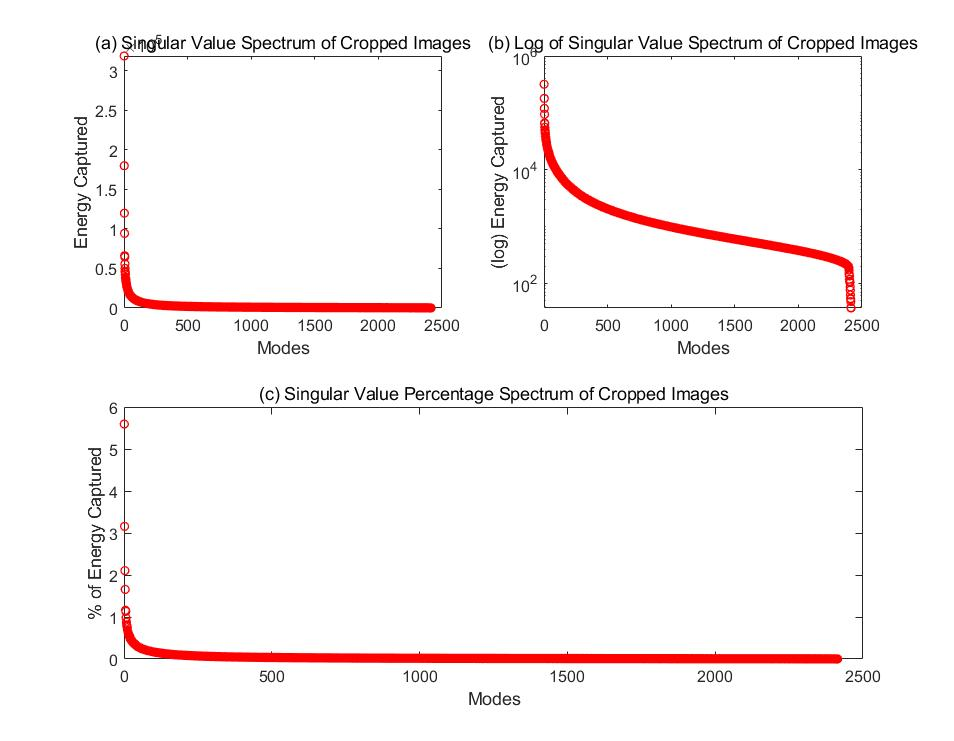
\includegraphics[scale=0.25]{S1.jpg}
\caption{Singular Value Spectrum($\Sigma$) for ((a) energy captured (b) log of energy captured (c) \% of energy captured) from cropped images}
\end{center}
\end{figure}
Figure 1 shows the amount (and percentage) of energy captured by each mode. There are "2414" modes but the energy captured drops down significantly after about 250-th node. Note that this is interpretation of $\Sigma$ matrix, which gives information about eigenvalues.
\begin{figure}[H]
\begin{center}
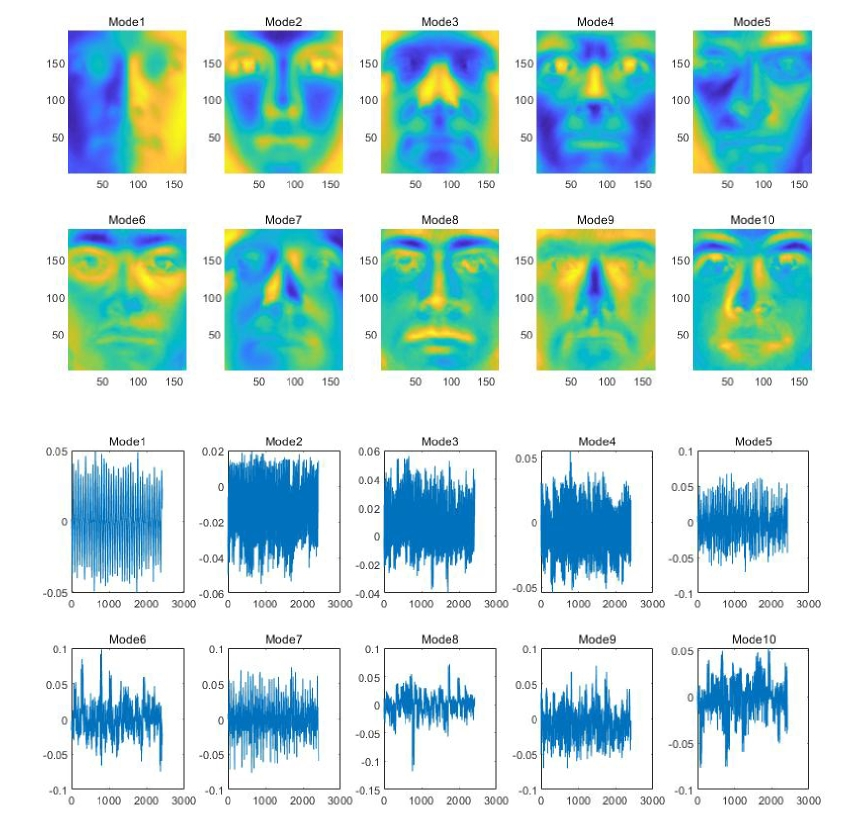
\includegraphics[scale=0.40]{U1V1.jpg}
\caption{Eigenfaces(U) (above) and projection eigenvector(V) (bottom) for first ten modes of cropped images}
\end{center}
\end{figure}
In Figure 2, we can see the interpretation of U and V, where U is the ``eigenface'' whose columns give information about where should each pixels be at and their intensity. But this matrix lacks details like lighting, skin colors and other facial features, where can be complemented by V, which gives information about details especially ``how much'' should a specific feature present. U and V together forms an orthonormal basis for our matrix.

\begin{figure}[H]
\begin{center}
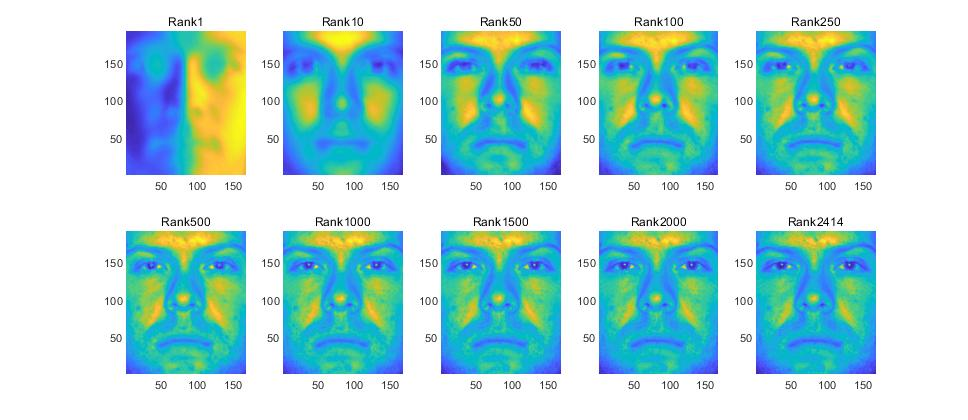
\includegraphics[scale=0.42]{Ares.jpg}
\caption{Reconstructed first cropped face image with varying rank levels}
\end{center}
\end{figure}
As we can see in Figure 3, the uncropped face image reconstruction of varying ranks. Clearly, there is a significant ``spike'' in terms of details occurred in rank 100. From this on, facial reconstruction looks almost the same as the original image (rank 2414). 
\begin{figure}[H]
\begin{center}
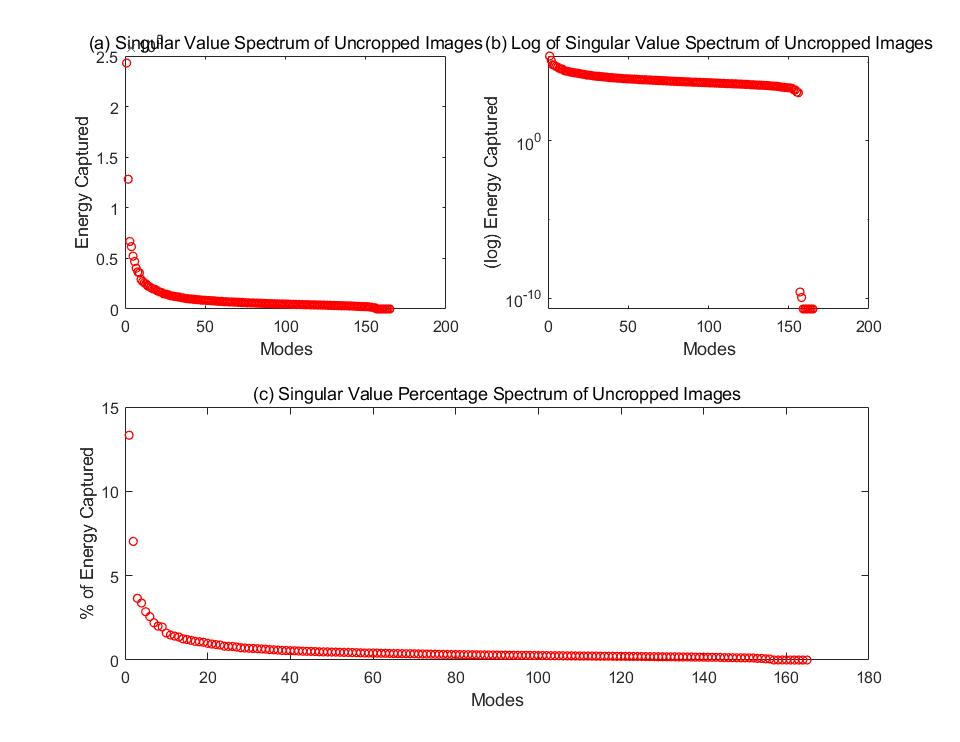
\includegraphics[scale=0.25]{S2.jpg}
\caption{Singular Value Spectrum($\Sigma$) for ((a) energy captured (b) log of energy captured (c) \% of energy captured) from uncropped images}
\end{center}
\end{figure}
Now we apply the same principle to uncropped images and start to notice that energy captured by each mode was quite ``average'', meaning that it possibly will take us comparatively high rank to approximate the image.
\begin{figure}[H]
\begin{center}
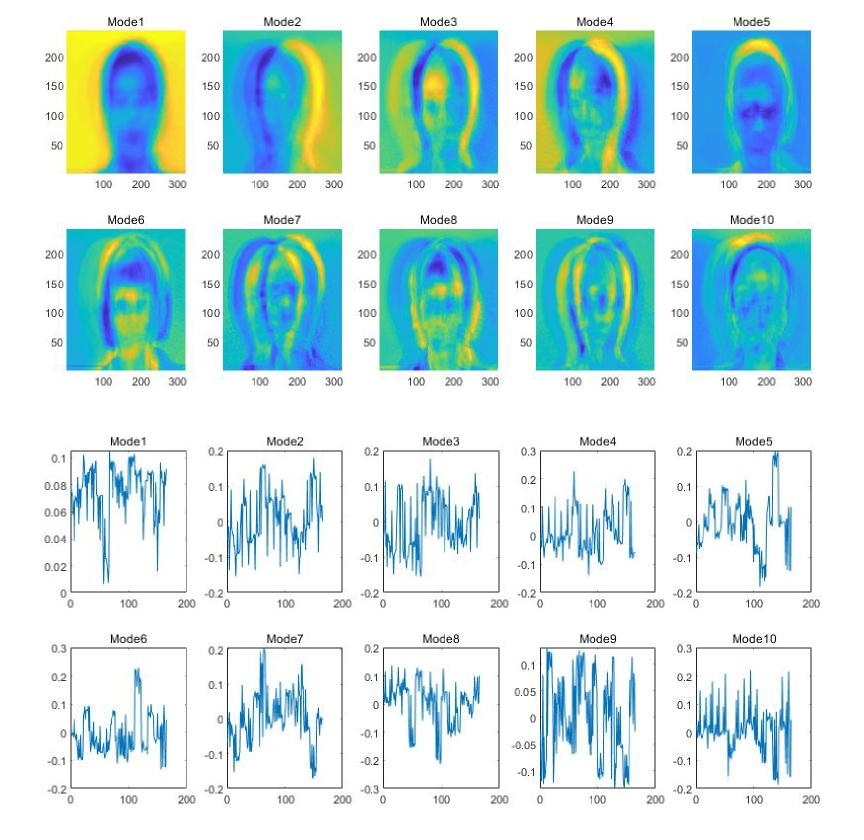
\includegraphics[scale=0.40]{U2V2.jpg}
\caption{Eigenfaces(U) (above) and projection eigenvector(V) (bottom) for first ten modes of uncropped images}
\end{center}
\end{figure}
Figure 5 clearly shows that U and V for uncropped images lose resolution remarkably, there's hardly any facial features presented in the first ten modes. This can be verified by the previous graph that mode-efficiency in terms of energy is very low in uncropped images.  
\begin{figure}[H]
\begin{center}
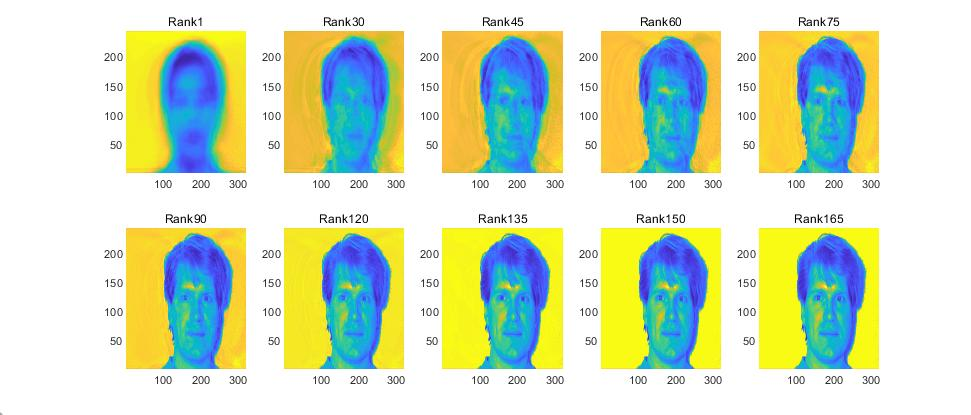
\includegraphics[scale=0.42]{Mres.jpg}
\caption{Reconstructed first uncropped face image with varying rank levels}
\end{center}
\end{figure}
Figure 6 helps us to future illustrate that cropping is necessary  for the image reconstruction on a specific study object. We can see that it only takes about "100" ranks out of "2414" to approximate the cropped face but "90~120" ranks out of "165" to restore an uncropped one.
\subsection{Music Genre Identification}
\subsubsection{Test 1}
\begin{figure}[H]
\begin{center}
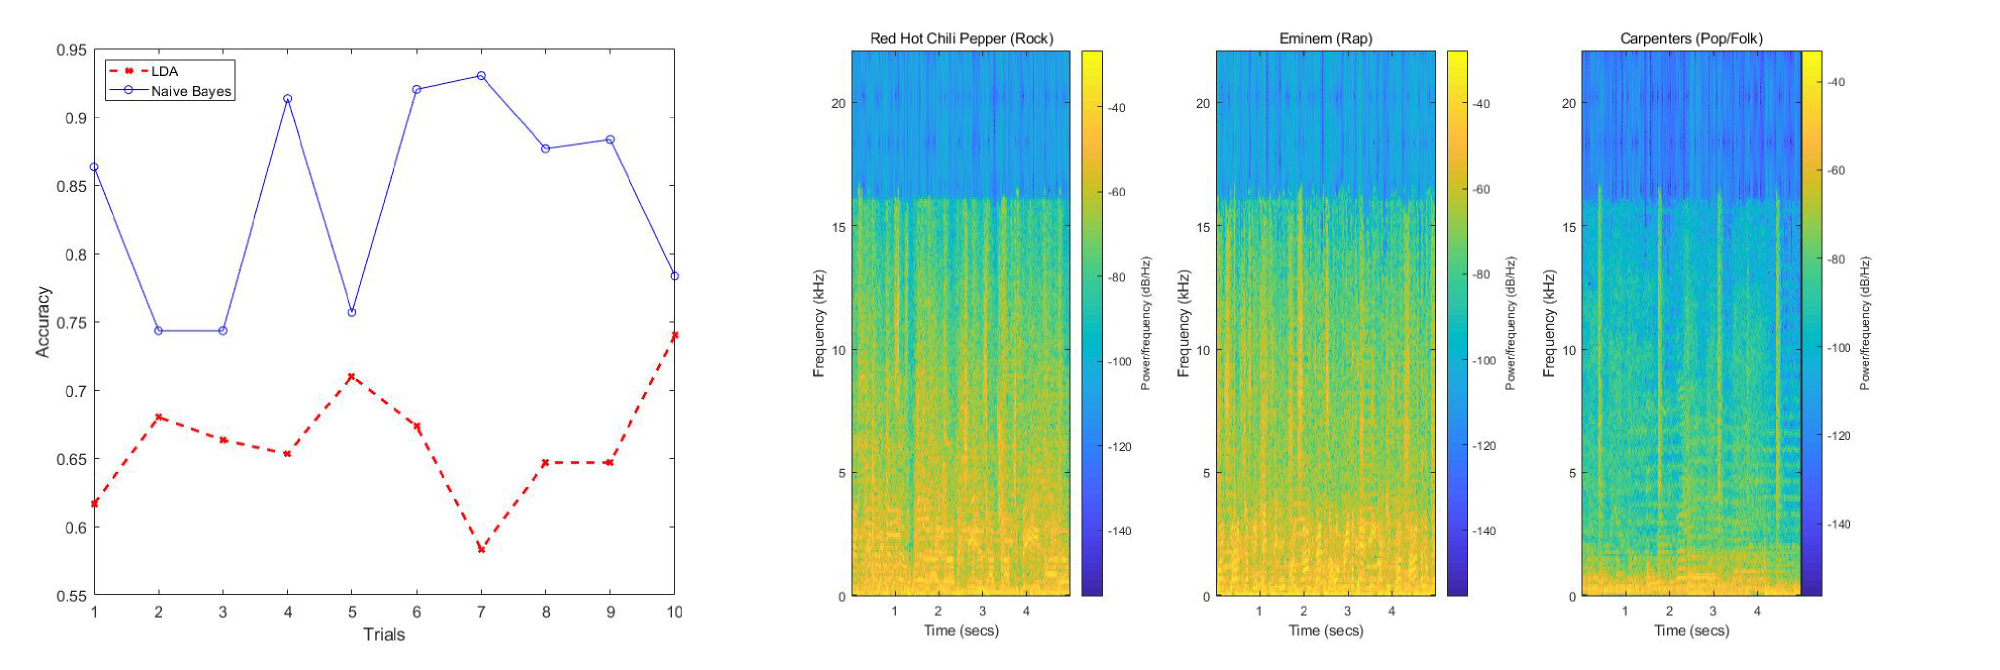
\includegraphics[scale=0.20]{t1.jpg}
\caption{Prediction Accuracy Plot of two classifying algorithms(left) and spectrograms (right) of sampled songs of same bands in different genres}
\end{center}
\end{figure}
We can observe from figure 7 that the na\"ive Bayes Classification works better than LDA does when songs are from the same three bands regardless different genres. It is clear that although songs may vary in style or genre, bands tend to have a ``unique'' frequency signature in their songs. Also, as mentioned in previous sections that Bayes classifier is a family of classifying methods, study objects that preserve common features can be better predicted and recognized.\\
The LDA, on the other hand, performs not as good as Bayes in this case because it relies on the independence of variables and thus can be not so good with dealing categorical variables.
\subsubsection{Test 2}
\begin{figure}[H]
\begin{center}
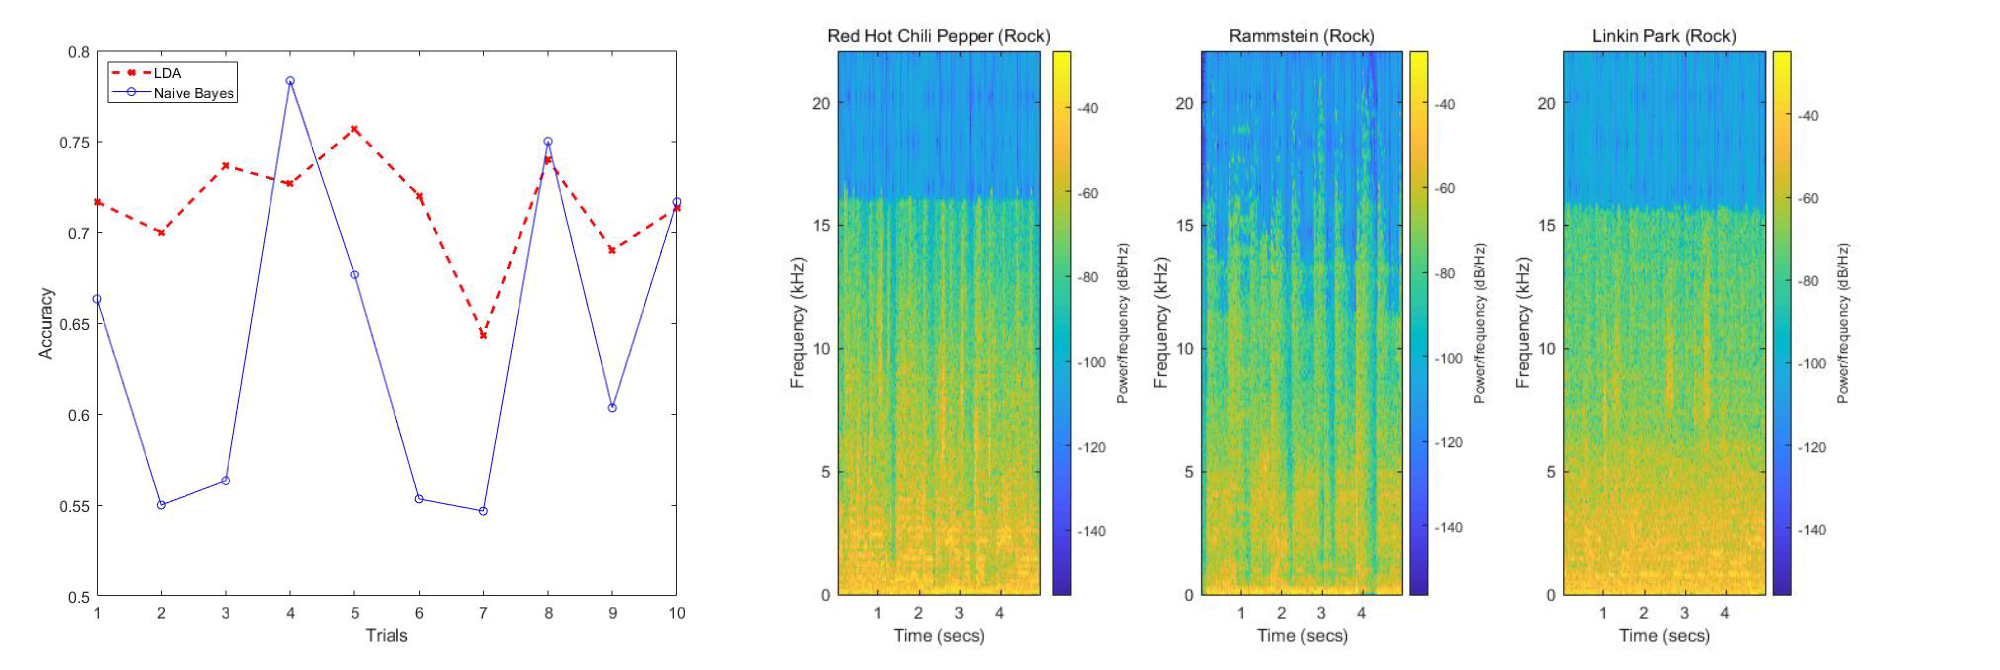
\includegraphics[scale=0.20]{t2.jpg}
\caption{Prediction Accuracy Plot of two classifying algorithms after ten runs (left) and spectrograms (right) of sampled songs in same genres of different bands}
\end{center}
\end{figure}
The accuracy of Bayes method drops down remarkably in this case, possibly due to the lack of variation in category as these "9" pieces of songs are of the same genre.\\ There are a couple of successful prediction that is quite precise, but rest of the trials are not so significant. Now, LDA in this case performs much better that Bayes does. It can be speculated that as we are analysing features of individual songs from same bands, we rely more on independent variables so that Bayes will constantly fail or lose much accuracy in reorganizing patterns and predicting.

\subsubsection{Test 3}
\begin{figure}[H]
\begin{center}
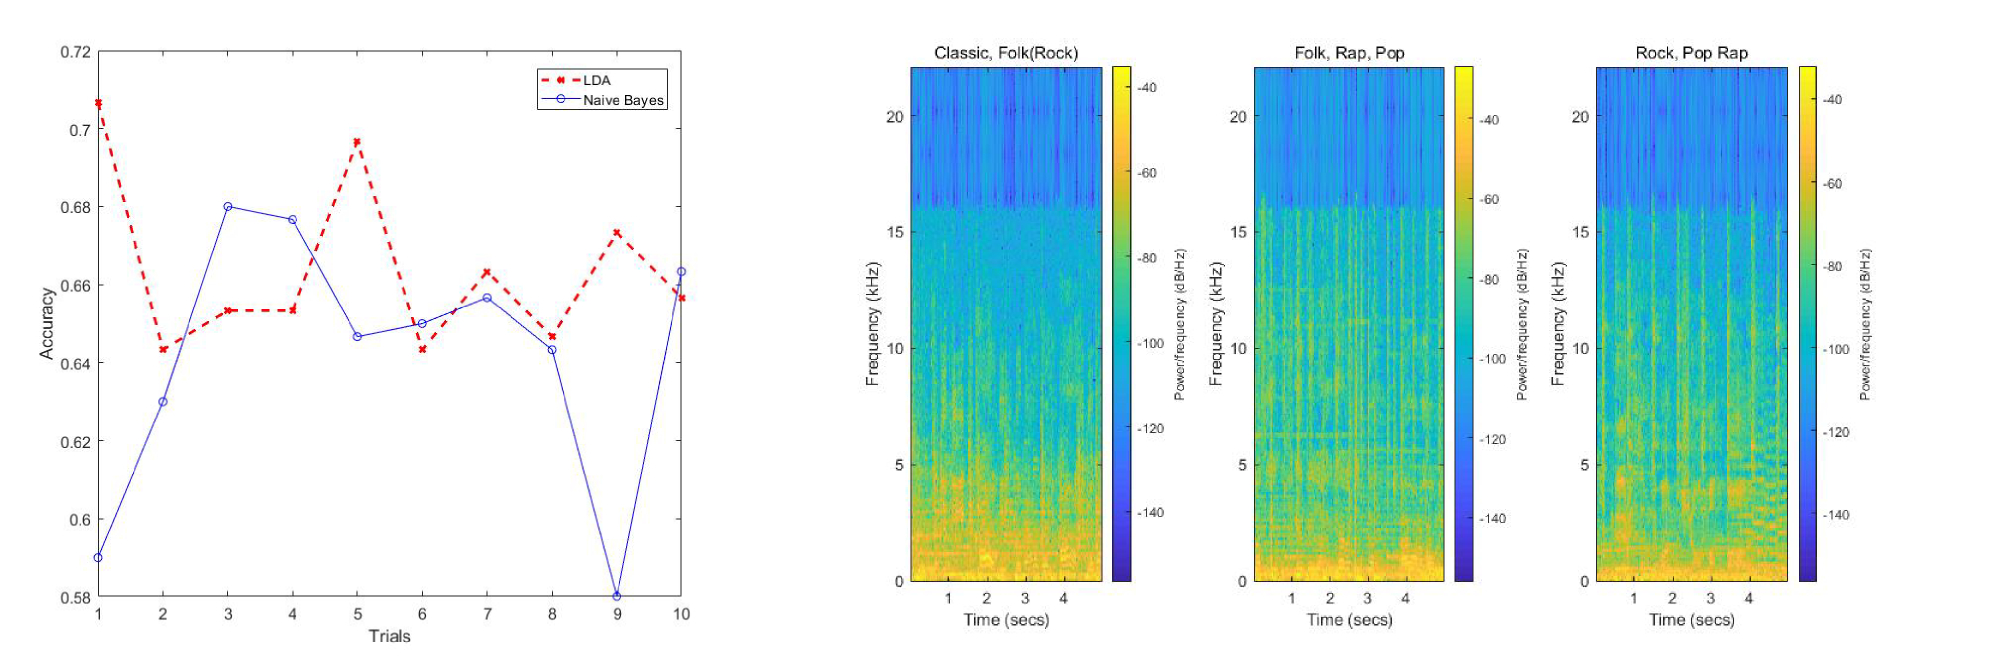
\includegraphics[scale=0.20]{t3.jpg}
\caption{Prediction Accuracy Plot of two classifying algorithms(left) and spectrograms after ten runs (right) of sampled songs of multiple artists and various genres}
\end{center}
\end{figure}
As we can see in Figure 8, accuracy for the Bayes classifier drops down yet again as genres and artists further mix up. Surprisingly, LDA results is quite assuring, which are relatively stable and is even capable of maintaining "71~72"\% of accuracy given that sample matrix of songs mixed up randomly.

\section{Summary and Conclusions}
In the first part, we studied the SVD analysis on image processing and discussed practical representation of $U, \Sigma \text{ and } V$. In particular, U and V forms an orthonormal basis that offers information of eigenface and significant details while S($\Sigma$) describes eigenvalues that imply the energy-efficiency of each mode. Moreover, we have explored the effect of image cropping and how such technique helps us to perform low-rank approximation.\\
We then studied different music genres and test if classifying methods can train and learn to identify music genres and found out that the Linear Discriminant Analysis has great potentials in maintaining pattern recognition accuracy and predicting while the Na\"ive Bayes classifier, despite of being very accurate in recognizing songs in the same category, relies heavily on the conditional probabilistic models and therefore failed to predict cases with more independent variables.


\begin{thebibliography}{3}
	\bibitem{582}
	J. Nathan Kutz. 2013.
	\textit{Data-Driven Modeling \& Scientific Computation}. p. 53-74
	
	\bibitem{mtlb}
	\textit{Matlab Documentation. Mathworks}; [2019 Mar 8]. \\https://www.mathworks.com/help/index.html

	\bibitem{svd}
	\textit{Singular Value Decomposition. Wikipedia}; [2019 Mar 8]. \\https://www.en.wikipedia.org/wiki/Singular\_Value\_Decomposition
	\bibitem{lda}
	\textit{Linear discriminant analysis. Wikipedia}; [2019 Mar 8]. \\https://www.en.wikipedia.org/wiki/Linear\_Discriminant\_Analysis
	\bibitem{nbc}
	\textit{Naive Bayes Classifier. Wikipedia}; [2019 Mar 8]. \\https://www.en.wikipedia.org/wiki/Naive\_Bayes\_Classifier

\end{thebibliography}


\section*{Appendix A: MATLAB functions used}
	\begin{itemize}
		\item \texttt{strcat}\\
		Concatenate strings horizontally
		\item \texttt{dir}\\
		List folder contents
		\item \texttt{imread}\\
		Read the image from the file specified by "filename"
		\item \texttt{repmat}\\
		"B = repmat(A,r1,...,""rN)" specifies a list of scalars, "r1,..,rN", that describes how copies of "A" are arranged in each dimension
		\item \texttt{svd}\\
		\texttt{[U,S,V] = svd(A)} performs a singular value decomposition of matrix \texttt{A}, such that \texttt{A = U*S*V'}
		\item \texttt{reshape}\\
		"B = reshape(A,sz)" reshapes "A" using the size vector, "sz"
		\item \texttt{audioread}\\
		"[y,Fs] = audioread(filename)" reads data from the file named "filename", and returns sampled data, "y", and a sample rate for that data, "Fs".
		\item \texttt{unidrnd}\\
		Generate discrete uniform random numbers.
		\item \texttt{spectrogram}\\
		Returns the short-time Fourier transform
		\item \texttt{gausswin}\\
		Returns an N-point Gaussian window in a column vector, "w"
		\item \texttt{classify}\\
		Returns the Classify Markov chain states
		\item \texttt{fitcnb}\\
		Returns a multiclass naive Bayes model "Mdl", trained by the predictors in table "Tbl" and class labels in the variable "Tbl"
		\item \texttt{predict}\\
		Predicts the output of K steps ahead using the measured input-output data of an identified model 
	\end{itemize}


\section*{Appendix B: MATLAB codes}
\subsection*{Extended Yale Faces B Database - Eigenfaces}
\lstinputlisting{h4a.m}
\subsection*{Music Genre Identification}
\lstinputlisting{h4b.m}
\subsection*{songClip.m}
\lstinputlisting{function.m}




\end{document}
